To address these complications in practice, a preliminary exercise was carried out which aimed to characterise the expected initial and final state interactions for the observation of a CC0\(\pi\) event in SBND. Alongside this, the potential backgrounds were also categorised in order to quantify their effect. 

This exercise also contributed to the initial construction of an anaylsis framework which will eventually be expanded to incorporate fully reconstructed simulations and multiple final state topologies. In the first stage of this exercise however, a MC sample of neutrino events was generated using the G00\_00b model configuration, described in Figure~\ref{tab:modelConfigs}, and a manual amount of smearing was applied to them along with energy cuts and an application of pionic impurities in order to loosely represent reconstructed events in SBND whilst training the analysis framework.  

\subsection{Smearing}

The Monte Carlo sample of SBND events was simulated using the Default+MEC GENIE model and the SBND flux, given in Figure~\ref{fig:SBNDFlux}. The quantites applied to the smearing, impurity additions and energy cuts are as follows \footnotemark,

\footnotetext{these quantities are in no way physically motivated. This entire anaylsis will eventually be implemented in a software framework which provides a dedicated reconstruction for liquid argon and so the smearing will not be a necessary step.}

    \begin{figure}[h!]
        \centering
        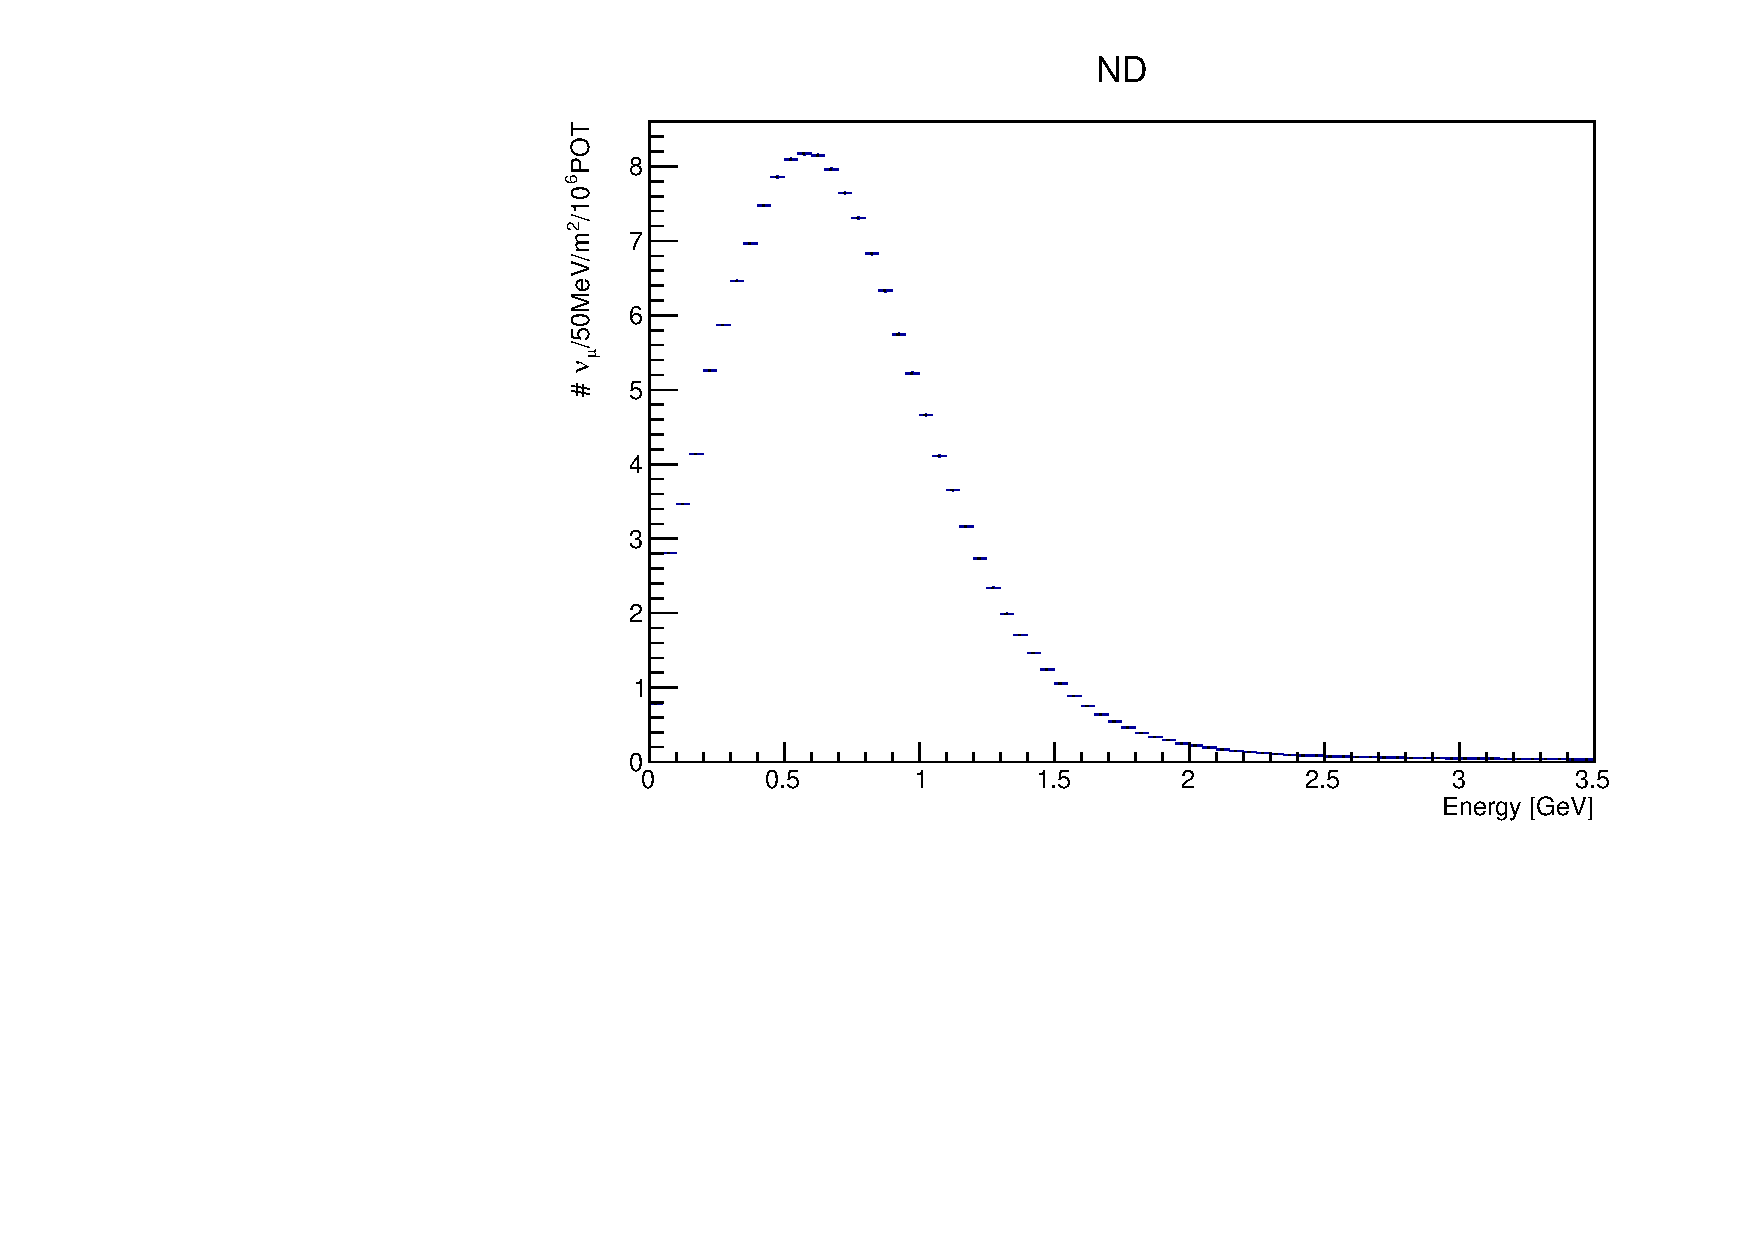
\includegraphics[width=.7\textwidth, trim=0 0 0 1cm, clip]{images/sbnd_flux.pdf}
        \caption{The flux of \(\nu_{\mu}\) at the short baseline near detector used to generate the neutrino events used throughout the following exercise}
        \label{fig:SBNDFlux}
    \end{figure}

\begin{itemize}
    \setlength\itemsep{.5em}
    \item Kinetic energy of the \(\mu\) : 10\%
    \item Opening angle of the \(\mu\) : 5\(^{\circ}\)
    \item \(\mu\) kinetic energy threshold > 50 MeV
    \item \(\pi^{\pm}\) kinetic energy threshold > 50 MeV
    \item Proton kinetic energy threshold > 50 MeV
    \item NC \(\pi^{\pm} \Leftrightarrow \mu\) mixup : 20\% of \(\pi^{\pm}\)
\end{itemize}

To smear the angular quantities, a random point was chosen from a Gaussian distribution about the true angle with a standard deviation of 5\(^{\circ}\). Since the cosine of this angle was the variable of interest, if the smeared angle was below 0\(^{\circ}\) the cosine of such a value would still be physically viable. However, a value of kinetic energy below 0 is not physically possible - since this implies the outgoing particles are travelling in the reverse direction to an interaction which occurred between a forward-going neutrino and a stationary nucleon. In this case, a lognormal distribution was used to randomly generate a kinetic energy with the true value as the mean, and a standard deviation of 10\%. 

The definition of a point on a lognormal distribution is given by equations~(\ref{eq:lognorm}), (\ref{eq:lognorm1}) and~(\ref{eq:lognorm2}) and is shown entirely generally for 100,000 data points about a mean of 10 and a variance of 0.5 in Figure~\ref{fig:logNorm}.

    \begin{equation}\label{eq:lognorm}
        X = e^{(\mu + \sigma)}
    \end{equation}

    \begin{equation}\label{eq:lognorm1}
        \mu = \ln \left( \frac{m}{\sqrt{1 + \frac{v}{m^2}}} \right)
    \end{equation}

    \begin{equation}\label{eq:lognorm2}
        \sigma = \sqrt{\ln \left( 1 + \frac{v}{m^2} \right) }
    \end{equation}
    
    where \( m \) is the mean, \( v \) is the variance or standard deviation squared and X is the smeared data point.   

    \begin{figure}[h!]
        \centering
        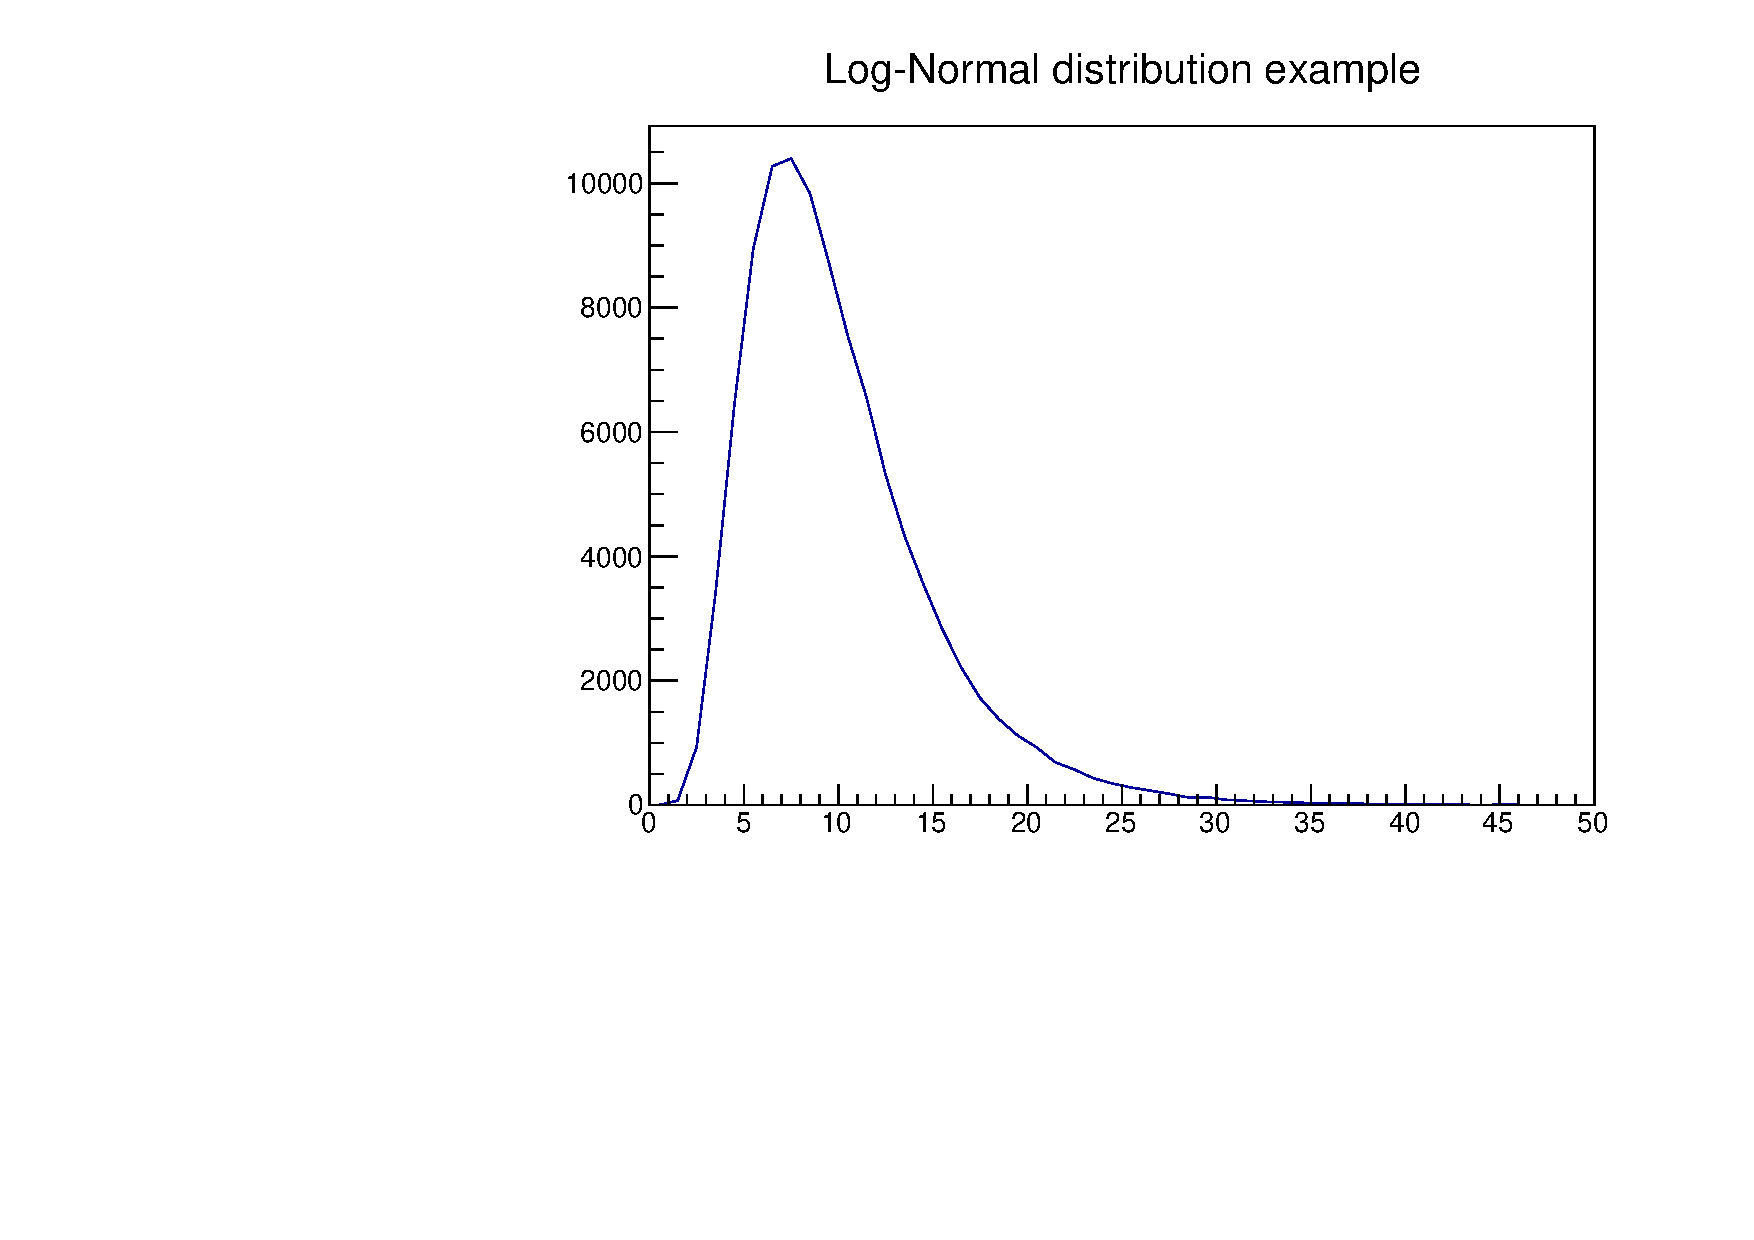
\includegraphics[width=.7\textwidth, trim=0 0 0 1cm, clip]{images/log_norm.pdf}
        \caption{An entirely general lognormal distribution, this is used to calculate smeared kinetic energies because the points never go below 0. T < 0 MeV is an unphysical value in a detector which accepts a forward-going neutrino beam.}
        \label{fig:logNorm}
    \end{figure}

In a CC0\(\pi\) interaction, the potential backgrounds within the detector will contaminate the signal for various reasons, including:

\begin{itemize}
    \item Low energy energy depositions of pions
    \item Mis-identification of pions
    \item ...
\end{itemize}

In this exercise, both the signal and background were split into potential contributing topologies in order to highlight the interaction characteristics within the detector and identify the channels which will be of interest in SBND. 

\subsection{Pre-FSI categorisation}

Using MC information, it is possible to characterise the signal based on the true, interaction-level event topology. Reconstruction within a detector would not allow for this, but studying these distributions gives and idea of how frequently pions get absorbed and other internucleon interactions take place.  

Figure~\ref{fig:preFSI} suggests that the dominant pre-FSI topology is a true CCQE event. It is also clear that multiple nucleon interactions, CCMEC, form a large portion of the CC0\(\pi\) final state topology. Charged current resonant and other 1\(\pi\) interactions contribute less, but are not negligable which suggests pions may frequently be emitted initially but never escape the nucleus.  

\begin{figure}[h!]
    \centering
    \begin{tabular}{cc}
        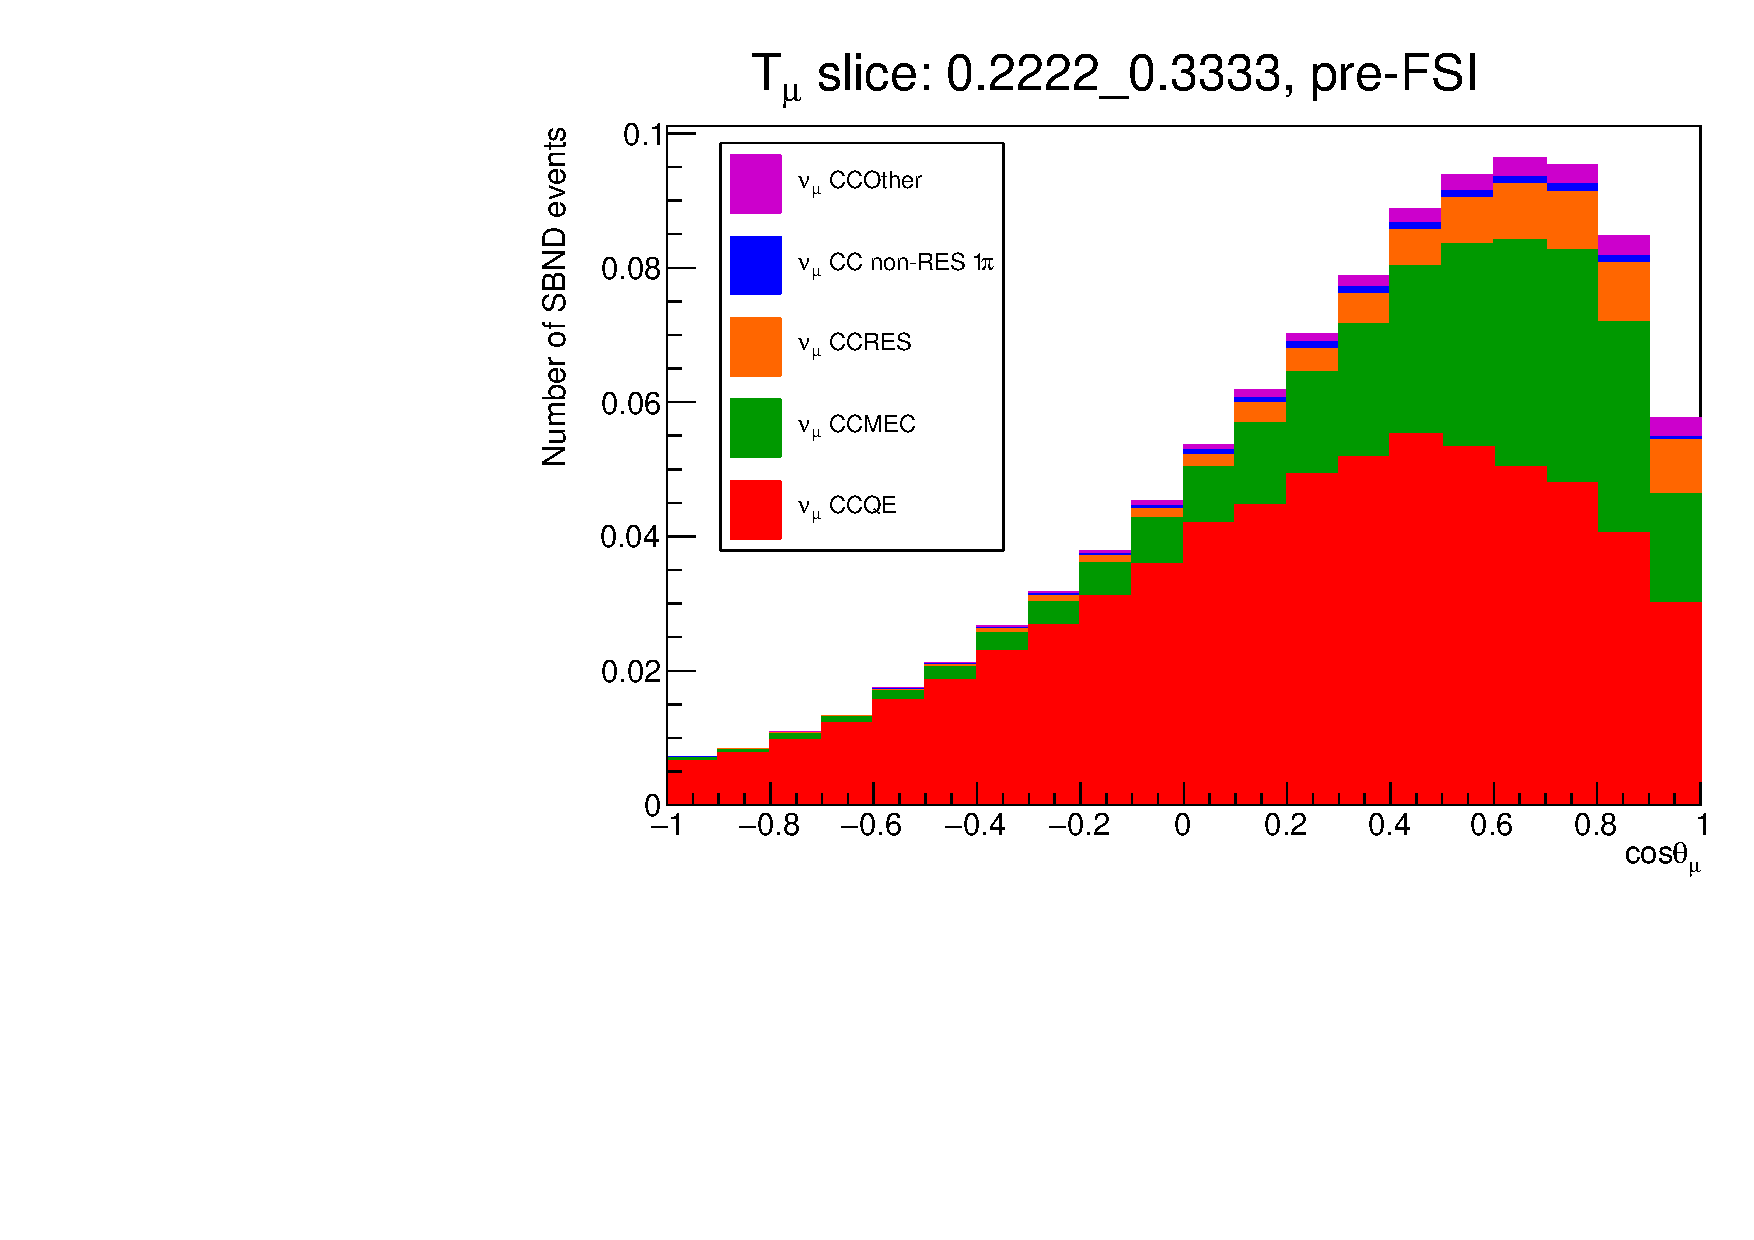
\includegraphics[width=.49\textwidth, trim=0 0 0 1.2cm, clip]{images/Pre_FSI_Tmu_slice_02222_03333.pdf}
        &
        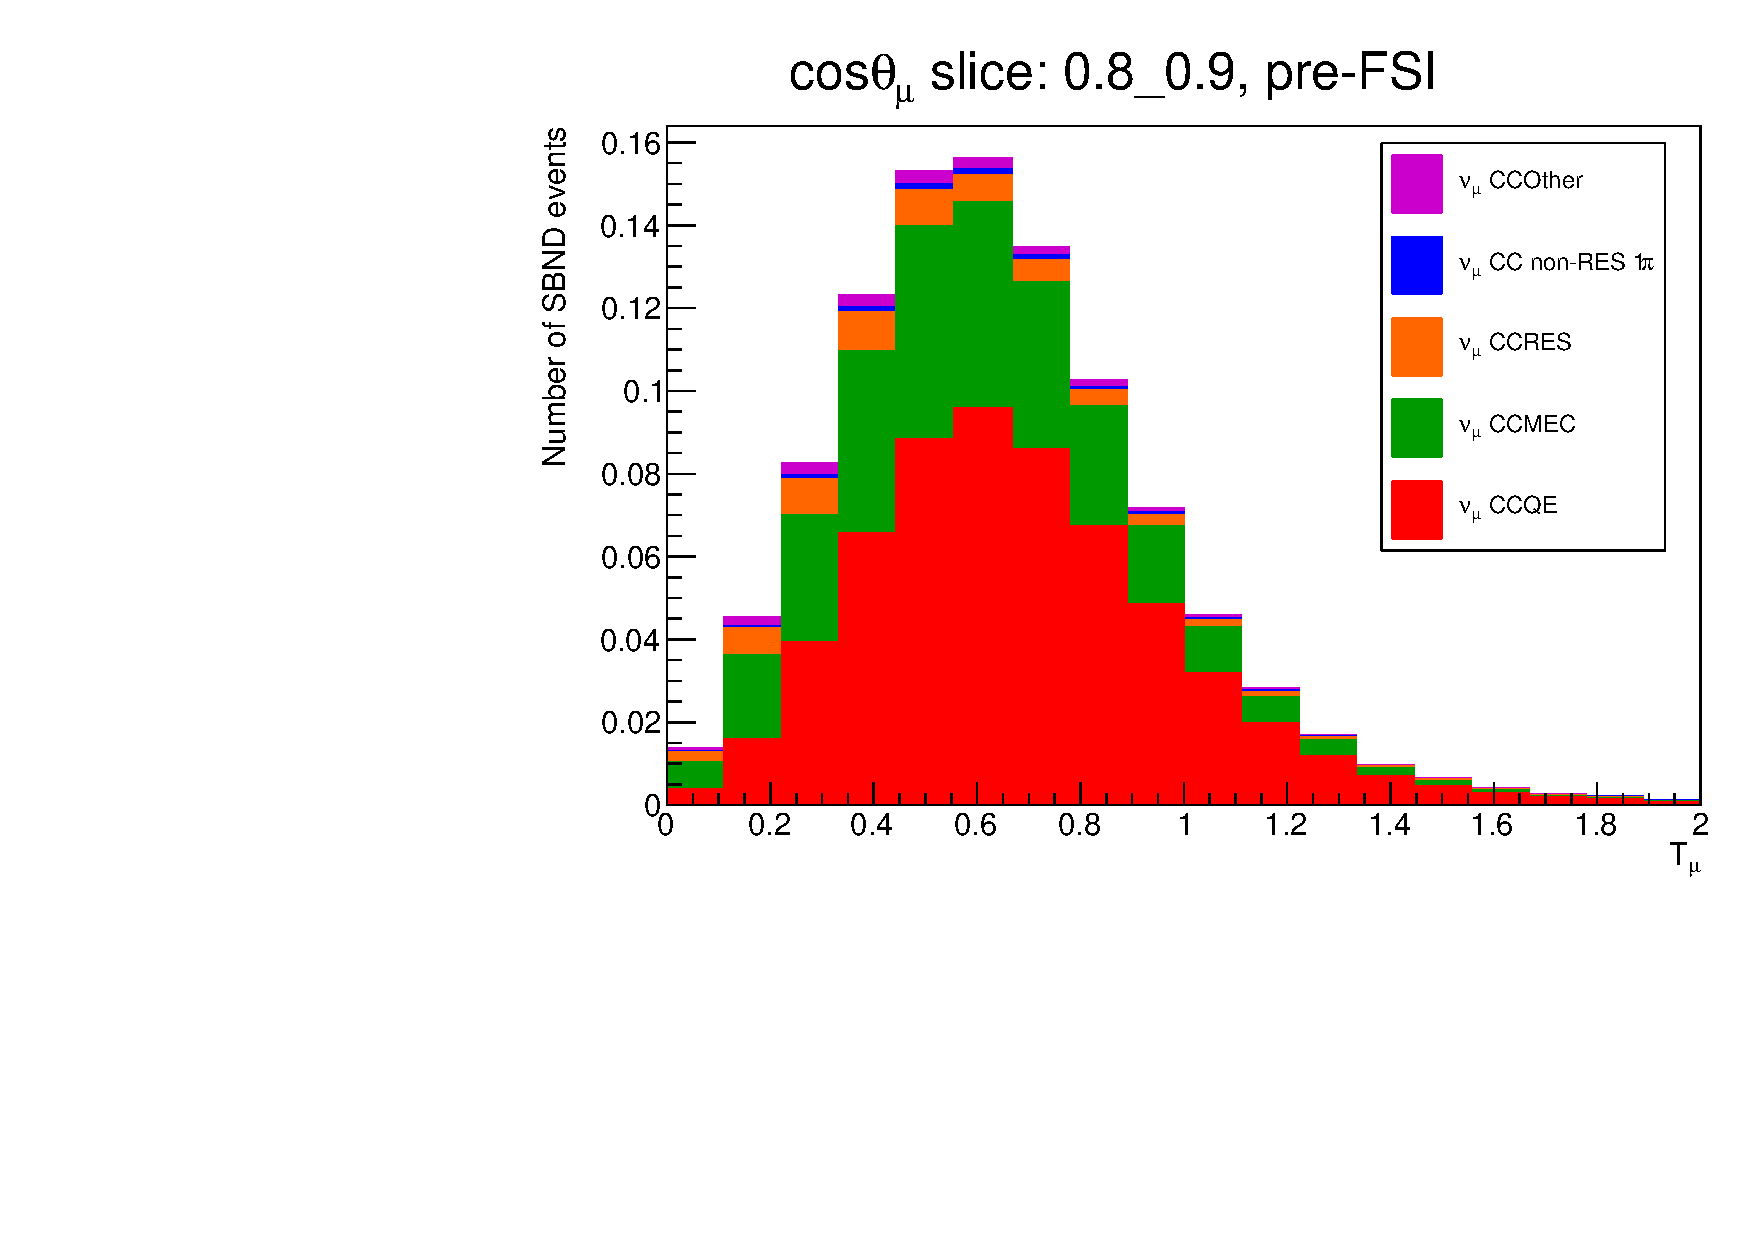
\includegraphics[width=.49\textwidth, trim=0 0 0 1.2cm, clip]{images/pre_FSI_cosmu_slice_08_09.pdf}
    \end{tabular}
    \caption{Area normalised muon kinetic energy and opening angle slices (left and right respectively) of the manually-reconstructed 2D distribution for CC0\(\pi\) events. These slices have been split into various pre-final state interaction topologies in order to build a picture of the likely contributing factors to an observed CC0\(\pi\) event: Charged current quasi-elastic (CCQE), charged current meson exhange current (CCMEC), charged current resonance (CCRES), changed current non-resonant single pion (CC non-RES 1\(\pi\)) and other charged current interactions. }
    \label{fig:preFSI}
\end{figure}

\subsection{Post-FSI categorisation}

The topologies chosen for study in the signal were based on the number of protons in the final state. Since the CC0\(\pi\) interaction only involves a neutrino and one or more nucleons, determining the number of nucleons involved in the initial interaction is the main source of interest in the study of this topology.

The backgrounds were split into all other possible interactions which could take place in the detector, with 10\% of charged current and 20\% of neutral current interactions being accepted as backgrounds - these acceptances are chosen to be low due to the high resolving power of SBND, which should allow for good distinction between signal and background \footnotemark.

\footnotetext{Once again, the chosen percentage of backgrounds to include is not a physically motivated value, since this will be treated with much more care when external backgrounds such as cosmic and dirt events are included in the next stage of this anaylsis.}


\begin{figure}[h!]
    \centering
    \begin{tabular}{cc}
        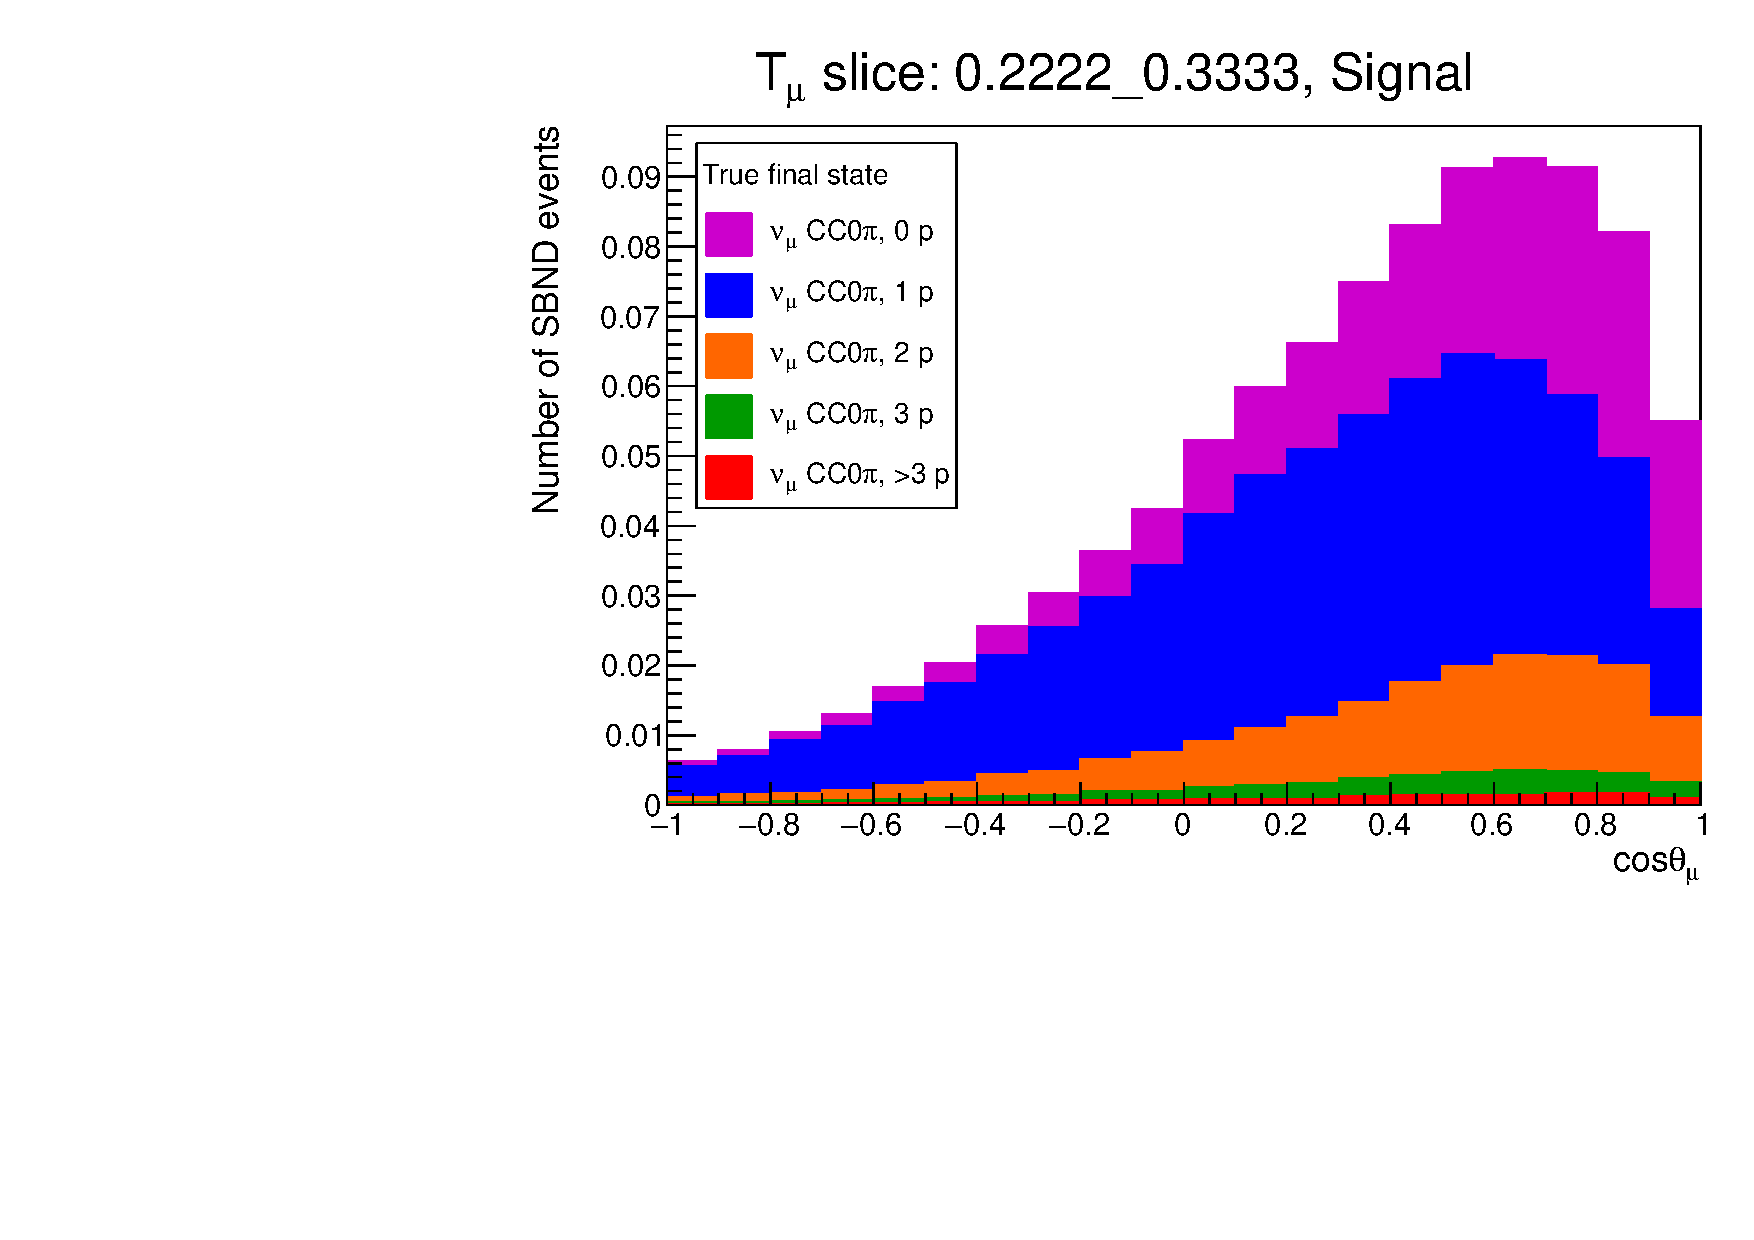
\includegraphics[width=.49\textwidth, trim=0 0 0 1.2cm, clip]{images/Signal_Tmu_slice_02222_03333.pdf}
        &
        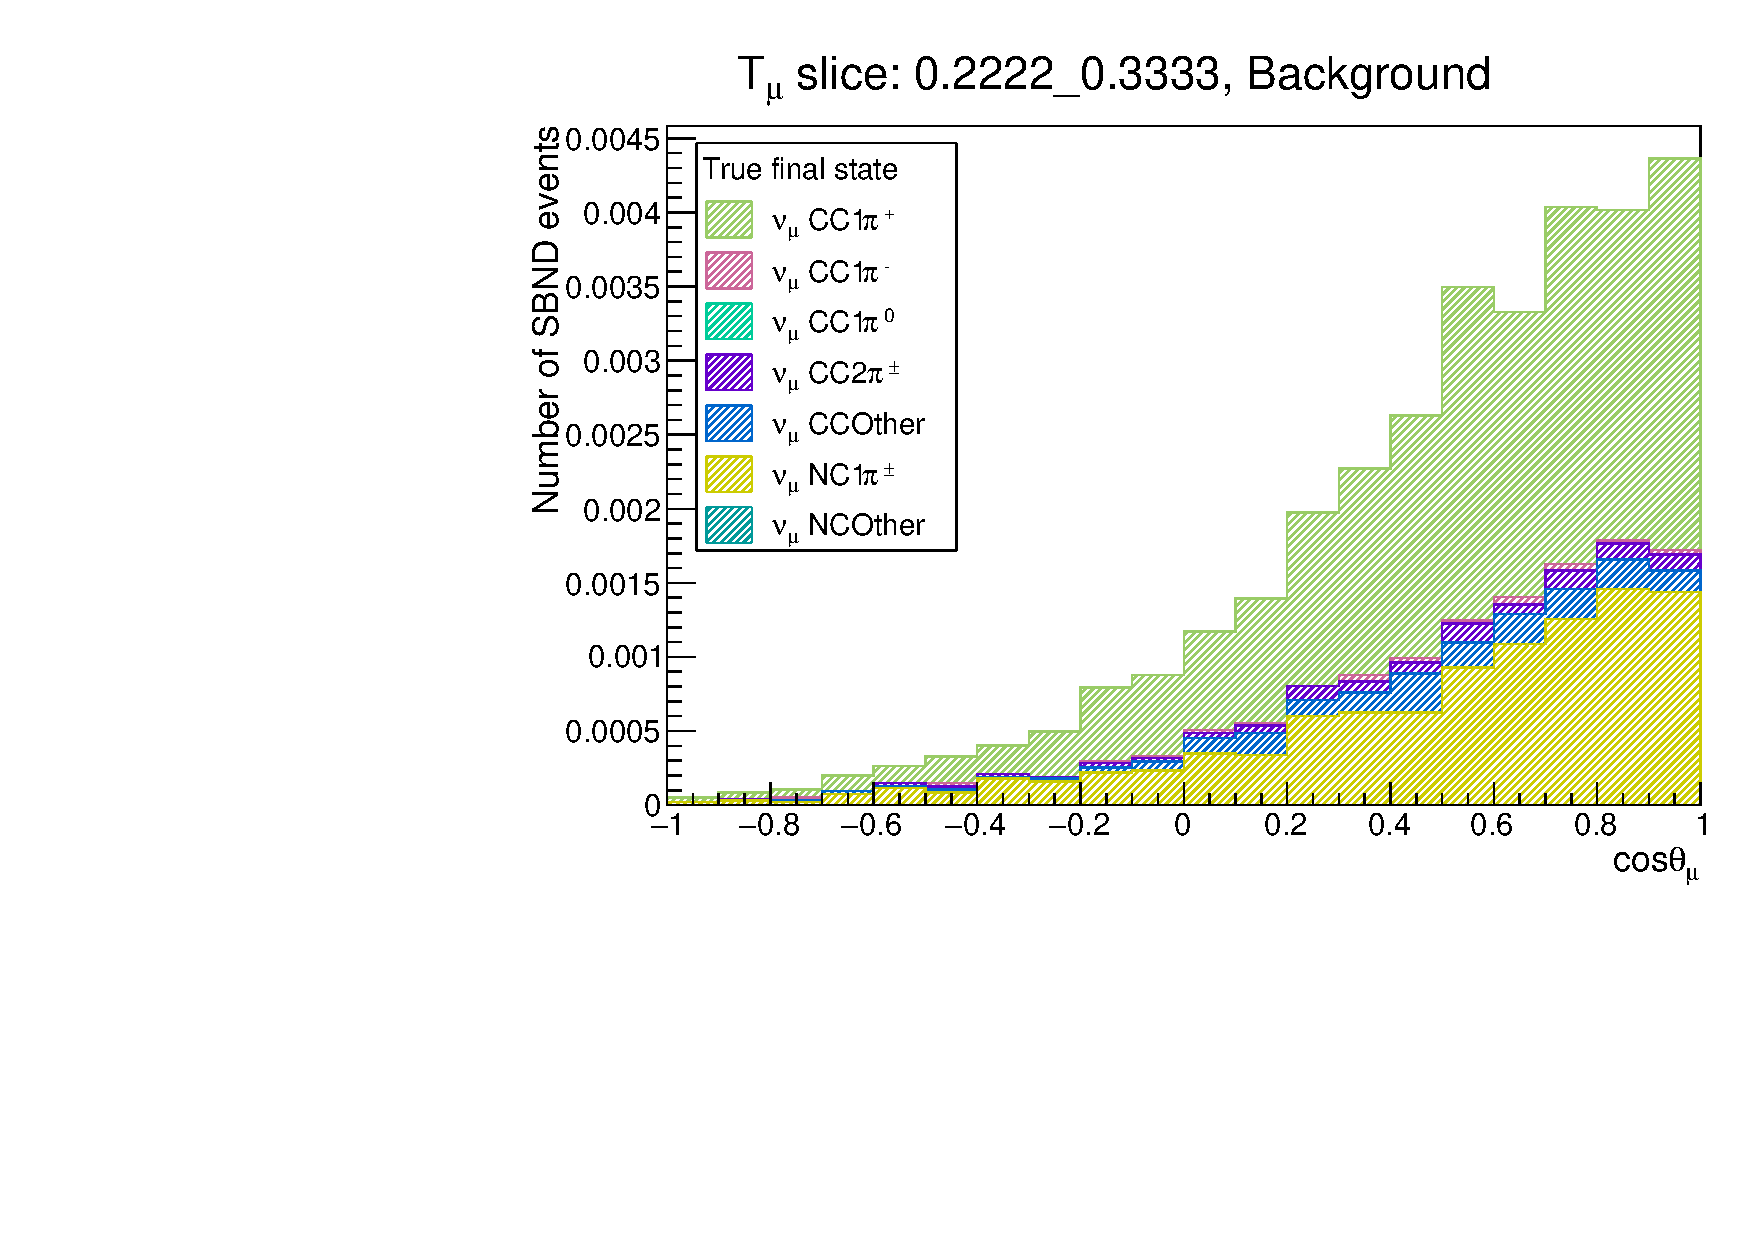
\includegraphics[width=.49\textwidth, trim=0 0 0 1.2cm, clip]{images/BG_Tmu_slice_02222_03333.pdf}
        \\
        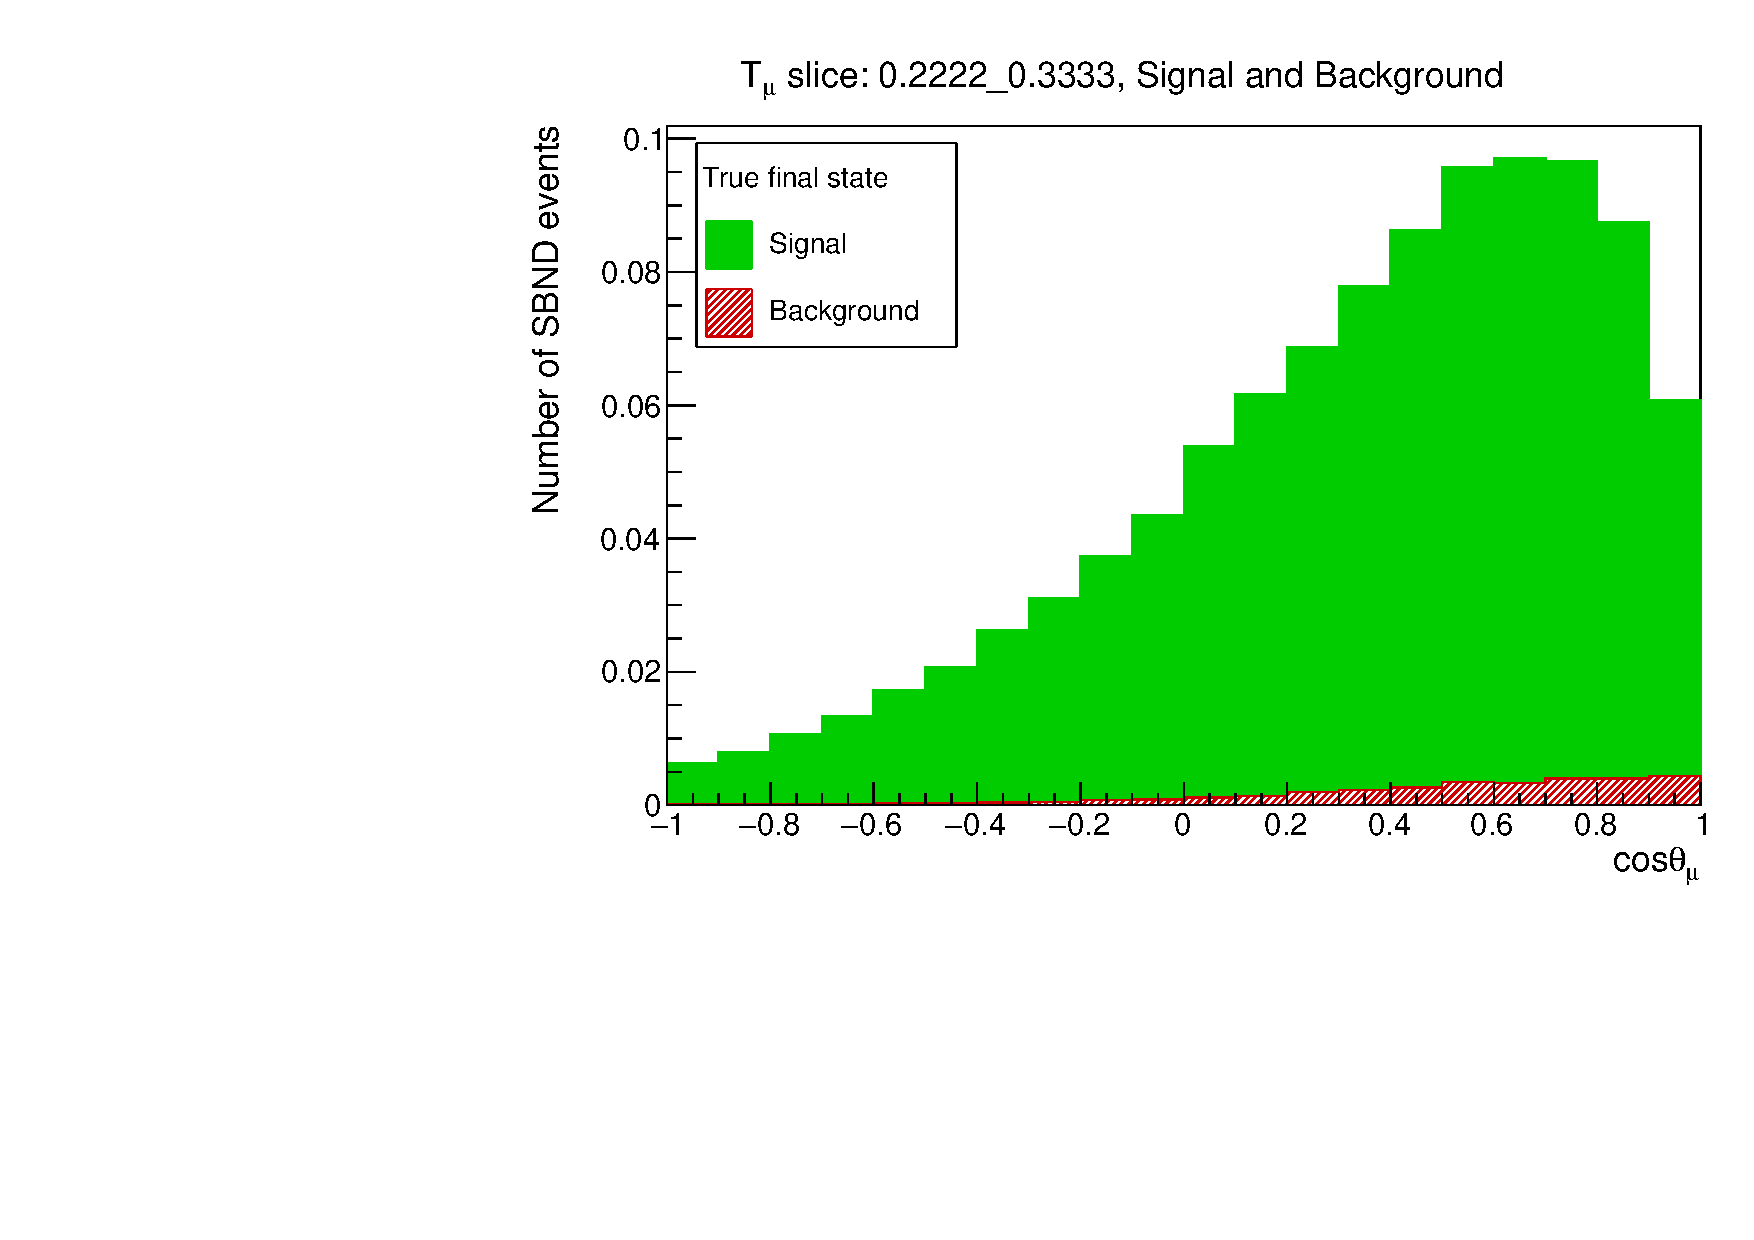
\includegraphics[width=.49\textwidth, trim=0 0 0 1.2cm, clip]{images/SBG_Tmu_slice_02222_03333.pdf}
        &
        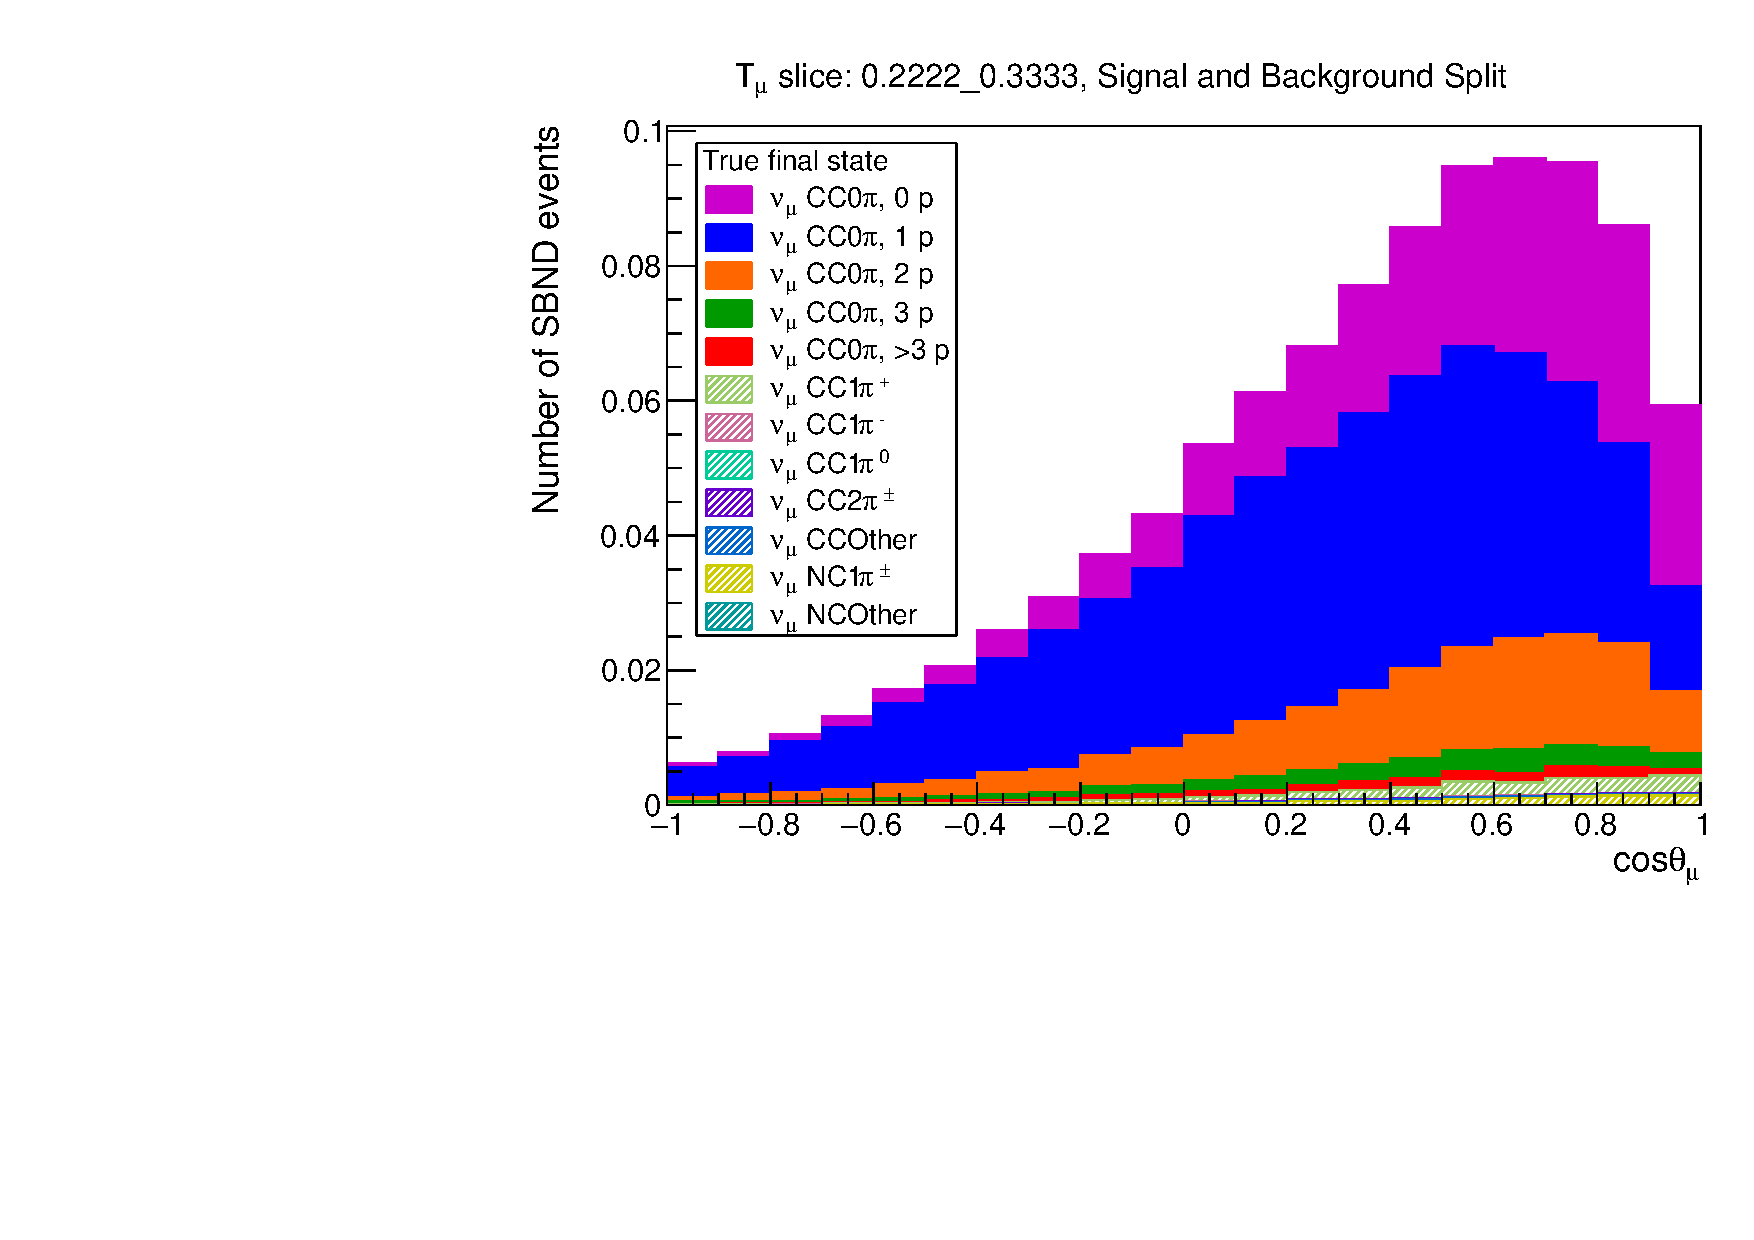
\includegraphics[width=.49\textwidth, trim=0 0 0 1.2cm, clip]{images/Split_SBG_Tmu_slice_02222_03333.pdf}
    \end{tabular}
    \caption{Top left: A breakdown of CC0\(\pi\) signal events into topolgies with different multiples of protons in the final state. Top right: Potential background event topologies. Bottom left: A comparison between signal and background shapes. Bottom right: All signal and background separated into topologies of interest.}
    \label{fig:postFSI_Tmu}
\end{figure}

The results shown in Figure~\ref{fig:postFSI_Tmu} are the signal and backgrounds for CC0\(\pi\) in SBND, characterised by splitting a slice of the 2D \(\mu\) opening angle - kinetic energy distribution into different event topologies.

The signal is split into CC0\(\pi, n\) protons. Where \( 0 < n \) in order to observe the contribution of the \( n \) particle \( n \) hole (\( npnh \)) effect. 

The backgrounds are split into charged current events with a single pion in the final state, charged current events with 2 charged pions in the final state, other charged current events, neutral current events with a single charged pion in the final state and other neutral current events. There should be no contribution from other neutral current events - this was included as a way of validating the method. 

From these figures it is clear that the background topologies which will likely dominate in SBND for the CC0\(\pi\) interaction are CC 1\(\pi^{+}\) and NC 1\(\pi^{\pm}\). The signal is dominated by events with low numbers of protons, which is to be expected when using 50 MeV energy thresholds on all particles. An event with more final state particles will likely give less energy to the individual particles which would then not be seen in the detector. 

\subsection{Moving forwards}

Now that the signal and internal backgrounds events have been characterised, the analysis can be moved into the dedicated liquid argon software framework: LArSoft, which will incorporate the detector geometry, external background contributions, detector propagation effects and eventually full reconstruction. Before the full reconstruction is available however, more realistic smearing and impurity quantities will be determined in order to provide more accurate, manual reconstruction in the meantime.  

An extention to this exercise would be to compare the smeared/reconstructed predictions with existing data to draw comparisons in a more realistic situation. The chosen experiment for this is MiniBooNE, which had the same baseline and energy range as SBND will have. For this reason, the kinematics studied were the same as that of MiniBooNE: muon kinetic energy as a function of the opening angle of the final state particles. An example comparison between
MiniBooNE data and predictions made by GENIE is shown in Figure~\ref{fig:MBComp}. The binning was also replicated in this exercise for the same reasons.

\clearpage
